\documentclass[11pt,a4paper]{article}
%\usepackage[toc,page]{appendix}
\usepackage{graphicx}
\usepackage[a4paper]{geometry}
\usepackage{xcolor}
\usepackage{fancyhdr}
\usepackage{float}
\usepackage{setspace}
\usepackage[absolute]{textpos}
\usepackage{epstopdf}
%\usepackage[]{mcode} 	% To include matlab code
\usepackage{capt-of}
\usepackage{enumerate}
\usepackage{lastpage}
\usepackage{booktabs}
\usepackage{longtable}
\usepackage{array}
\renewcommand{\arraystretch}{1.5}

\usepackage[english]{babel}
\usepackage[utf8]{inputenc}
\usepackage{amsmath}
\usepackage{amsfonts}
\usepackage{graphicx}
\usepackage[colorinlistoftodos]{todonotes}
\usepackage{algorithm}
\usepackage{algpseudocode}

\usepackage{amsmath}
\usepackage{algorithm}
%\usepackage[noend]{algpseudocode}
\makeatletter
\def\BState{\State\hskip-\ALG@thistlm}
\makeatother

\usepackage{array} % Table
\usepackage{amsmath}
\usepackage{amsfonts}
\usepackage{amssymb}
\usepackage{eurosym}
\usepackage{textcomp}

%Tables
\usepackage{multirow}

% Header
\setlength{\headheight}{30pt}
\newgeometry{top=2.5cm, bottom = 1.5cm, left=2cm, right=2cm}
\pagestyle{fancy} 
\lhead{\includegraphics[height=0.9cm]{figures/{qt_logo}.jpg}}
%\lfoot{Group 4 - ``CASE"-HENK}
\cfoot{~}
\rfoot{Page \thepage ~of \pageref{LastPage}}

\usepackage{cleveref}
% Change cleveref reference eq. to equation same for figure
\crefname{equation}{equation}{equations}
\crefname{figure}{figure}{figures}
\crefname{table}{table}{tables}

% Change Section numbering to Problem 1
%\renewcommand{\thesection}{Problem \arabic{section}.}

\begin{document}
%\begin{titlepage}
%\vspace*{100pt}
%\begin{figure}
%\centering
%\includegraphics[width=0.5\textwidth]{figures/TUelogozondertekst}
%\end{figure}
%\begin{center}
%{ \huge \bfseries 4AT100 Automotive Systems Engineering Project\\[0.4cm] }
%\textsc{\Large Concept Project Plan}\\[0.5cm]
%
%\end{center}
%
%\vfill
%
%\renewcommand{\arraystretch}{1}
%
%\begin{flushleft} \large
%\begin{tabular}{l}
%Project Coordinators:\\
%Dr.Ir. A. van de Mortel-Fronczak (Asia) \\
%Dr.Ir. I. Barosan (Ion) \\
%\end{tabular}
%\end{flushleft}
%
%\begin{flushleft} \large
%\begin{tabular}{l l l l}
%Tutor: & & & \\
%L. Kefalidis (Lazaros) & & & \\
%& & & \\
%Authors:\hspace{30mm} 	& \hspace{35mm}	& \hspace{55mm} 	    		& 			\\
%S. Forno (Simone) 		& ​0978942		& T. de Mor\'ee (Tim)			& 0944052 	\\
%R.M.A. Goris (Rob) 		& 0808822		& T.M.A. van de Wiel (Thijs)	​& 0824530 	\\
%B.S. Haarsma (Bouke) 	& 0751757​		& H. Wils (Hielke) 				& 0807014 	\\
%\end{tabular}
%\end{flushleft}
%
%\begin{flushleft} \large
%\begin{tabular}{l}
%MSc. Programme Automotive Technology \\
%Eindhoven University of Technology \\
%\end{tabular}
%\end{flushleft}
%
%\begin{flushleft} \large
%\begin{tabular}{l}
%\today \hspace{8.4cm} Group 4 ``CASE"-HENK \\
%\end{tabular}
%\end{flushleft}
%
%\renewcommand{\arraystretch}{1.5}
%
%\end{titlepage}

\newgeometry{top=2.5cm, bottom = 3cm, left=2cm, right=2cm}

%\newpage
%
%\setcounter{tocdepth}{2}
%
%\tableofcontents
%\newpage


%------------------------------------------------

\section{Download} \label{sec:down}

Download Qt Creator from the official release at this link https://download.qt.io/official{\_}releases/qt/, and select version \textbf{5.6}. Lower versions can be unsupported and might not be able to work with the debugger. The specific version used for this documentation is \textbf{5.6.1}.\\
For Linux systems run the file \textbf{qt-opensource-linux-x64-5.6.1.run}, and follow the installation wizard straight to the end. This will install Qt Creator in your machine. \\
Test the application by launching it from the terminal, simply typing \textbf{qtcreator \&}. This erases the starting window, like the one seen below.

\begin{figure}[!htb]
	\center
	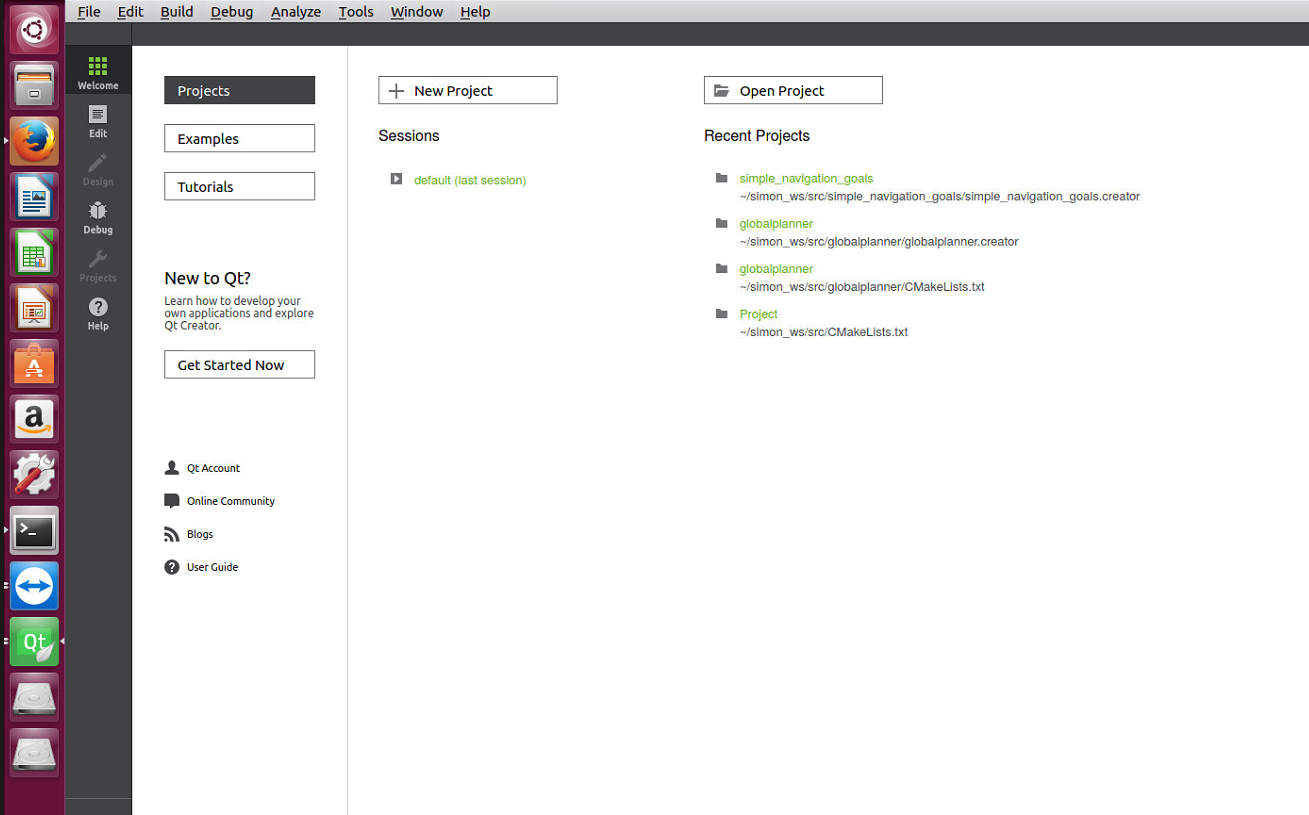
\includegraphics[width=1\textwidth]{figures/welcome.png}
	\caption{Welcome window opening the Qt Creator application}
	\label{fig:welcome}
\end{figure}

\section{Importing a catkin package} \label{sec:open}

Qt Creator is a versatile tool, naturally fitted to work with CMake build files. Any package under a \textbf{catkin workspace} can be built and run using Qt Creator, which resambles the functionality of the ROS \textbf{run} or \textbf{roslaunch} commands. \\
In order for Qt Creator to work in the catkin shell, the desired catkinized package (containing a \textbf{CMakeLists.txt and package.xml files}) should be imported into the application, by following the steps:
\begin{itemize}
\item Click on File \textrightarrow New File or Project. This will pop up the window shown in Figure \ref{fig:imp_1}.
\item Select Import existing projects and click Choose.
\item Give as Project Name the \textbf{exact} same name as the catkin package name you want to import. Browse to the path under the field Location. An example is visible in Figure \ref{fig:imp_2} In this case the name of the package is called \textbf{simple{\_}navigation{\_}goals} and the path is \textbf{simon{\_}ws/src/simple{\_}navigation{\_}goals}. Click Next.
\item Click Next to the following two windows that happear. Tick the checkbox \textbf{include} if the package contains header files in the include directory. 
\end{itemize}

\begin{figure}[!htb]
    \centering
    \begin{minipage}{.5\textwidth}
        \centering
        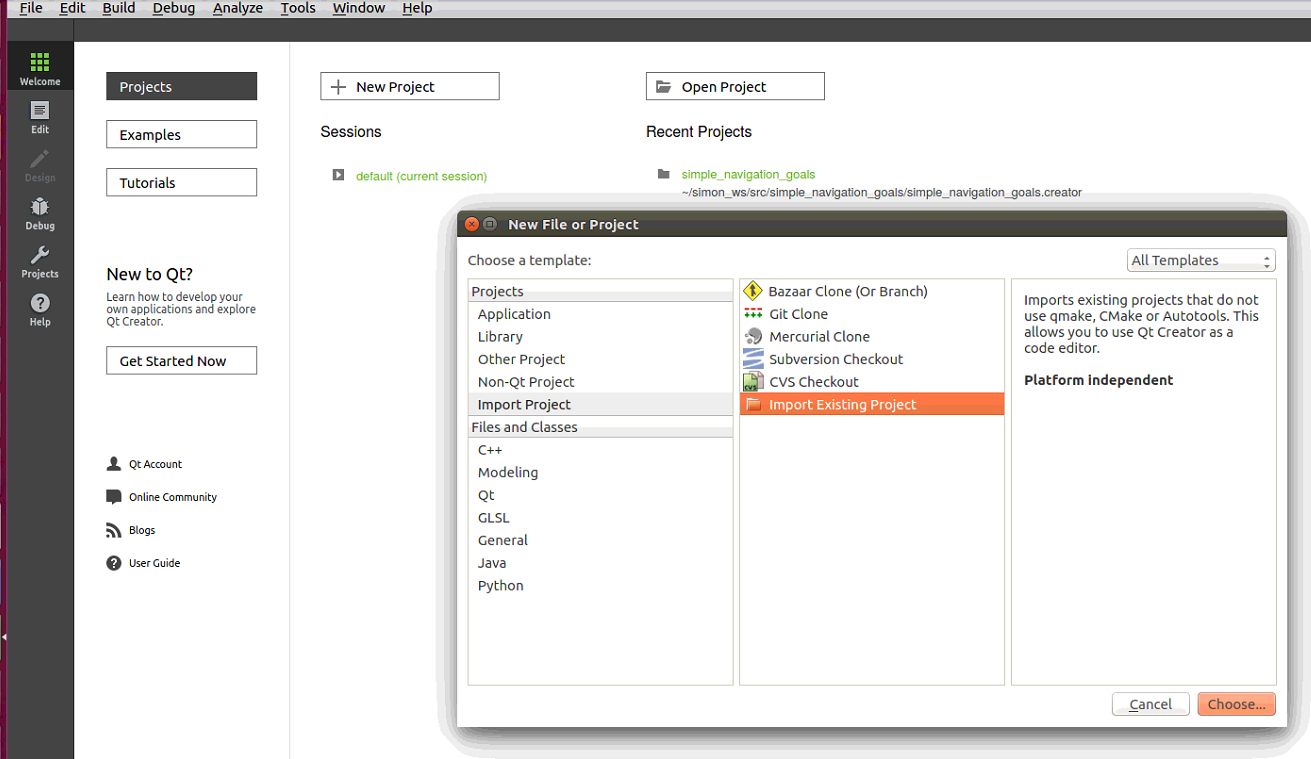
\includegraphics[width=0.9\linewidth, height=0.2\textheight]{figures/import_1}
        \caption{}
        \label{fig:imp_1}
    \end{minipage}%
    \begin{minipage}{.5\textwidth}
        \centering
        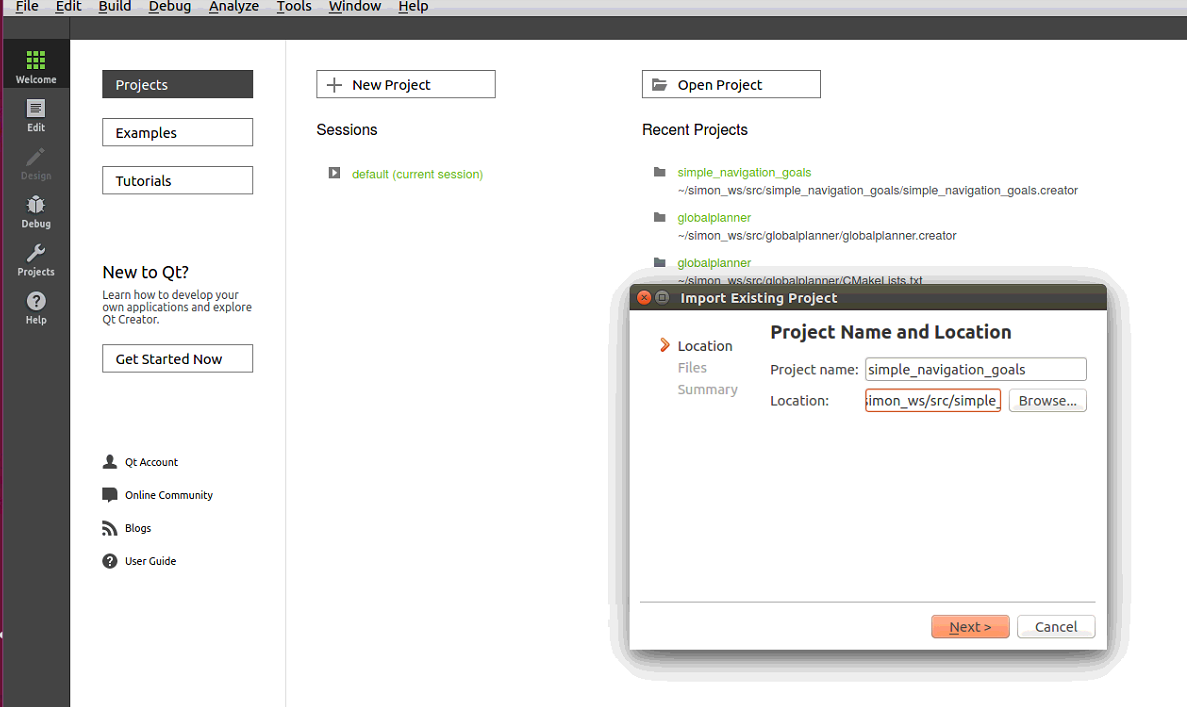
\includegraphics[width=0.9\linewidth, height=0.2\textheight]{figures/import_2}
        \caption{}
        \label{fig:imp_2}
    \end{minipage}
 \end{figure}


\section{Setting up the debugger to work with catkin} \label{sec:debug}

If the process has terminated succesfully till this point, you should see something similar to the top left corner of Figure \ref{fig:overall}. \\
To allow Qt Creator to build and run the package, the build and run settings should resamble the ones in Figure \ref{fig:build} and Figure \ref{fig:run}.

\begin{figure}[!htb]
	\center
	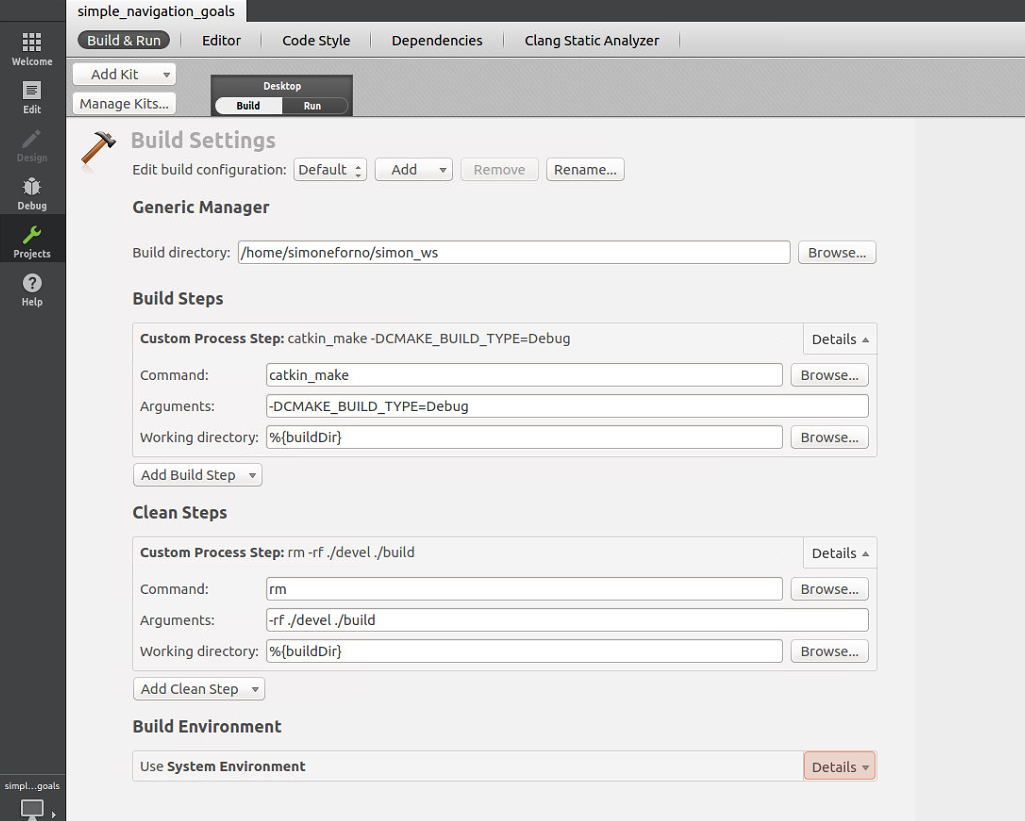
\includegraphics[width=0.8\textwidth]{figures/build_settings.png}
	\caption{Build settings of the catkin package}
	\label{fig:build}
\end{figure}

\begin{figure}[!htb]
	\center
	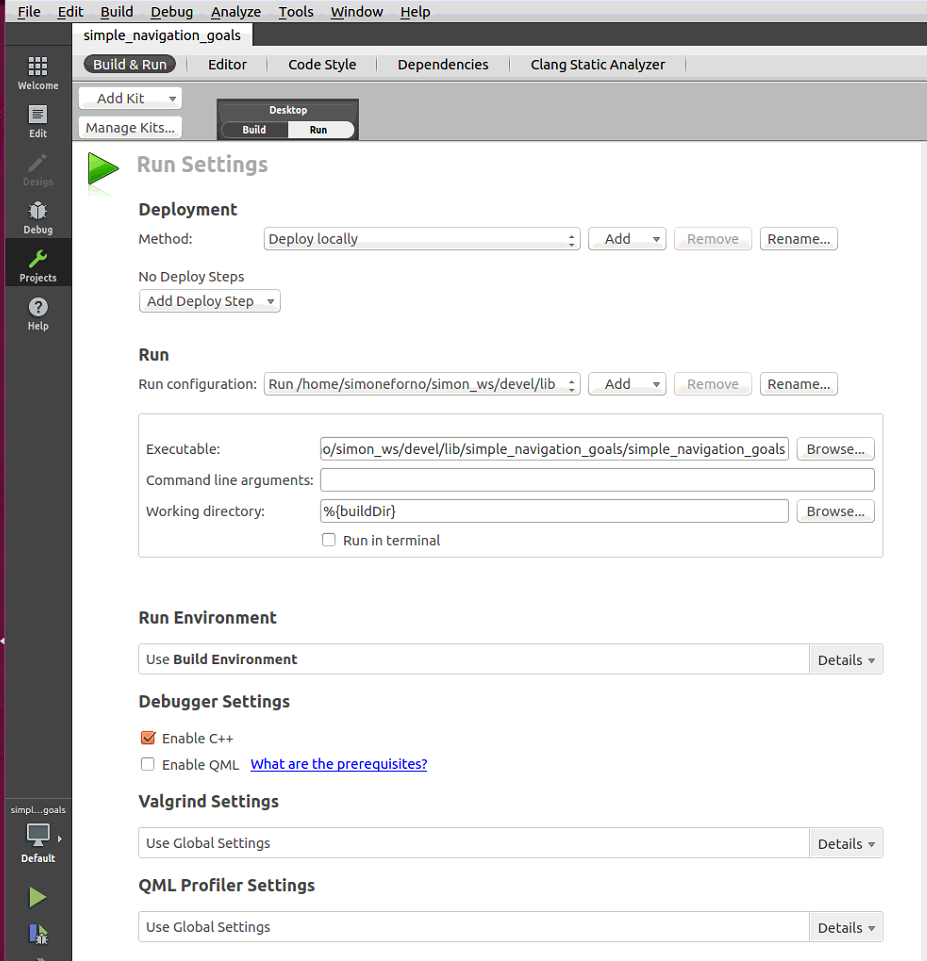
\includegraphics[width=0.8\textwidth]{figures/run_settings.png}
	\caption{Run settings of the catkin package}
	\label{fig:run}
\end{figure}

\subsection{Build settings}

\begin{itemize}
\item Change the Build Directory to the catkin root path and \textbf{do not} select the build folder under $workspace{\_}name/build$. 
\item Under Build Steps, delete the default existing Process Step and add a new Process step by clicking the \textbf{Add Build Step} tab \textrightarrow \textbf{Custom Process Step}. Fill in the build steps as in Figure \ref{fig:build}.
\item Do the same also for the \textbf{Clean Steps} tab, delete the default Process Step and fill in the fields as in Figure \ref{fig:run}.
\end{itemize}

\subsection{Run settings}

\begin{itemize}
\item Leave the \textbf{Deployment} part unchanged.
\item In the \textbf{Run} part, for the Run configuration part, click on Rename and browse to the \textbf{devel/lib} path of your catkin workspace.
\item Browse to the package Executable under the \textbf{lib} folder. Leave the remaining section as it is.
\end{itemize}

To debug the code, place breakpoints into the code and click on \textbf{Start Debugging} button, or \textbf{F5}. This will compile the package and create the targets. It is possible to visualize the variables in the top right panel, and see the changes by Stepping into the code, as see in Figure \ref{fig:overall}. 



\begin{figure}[!htb]
	\center
	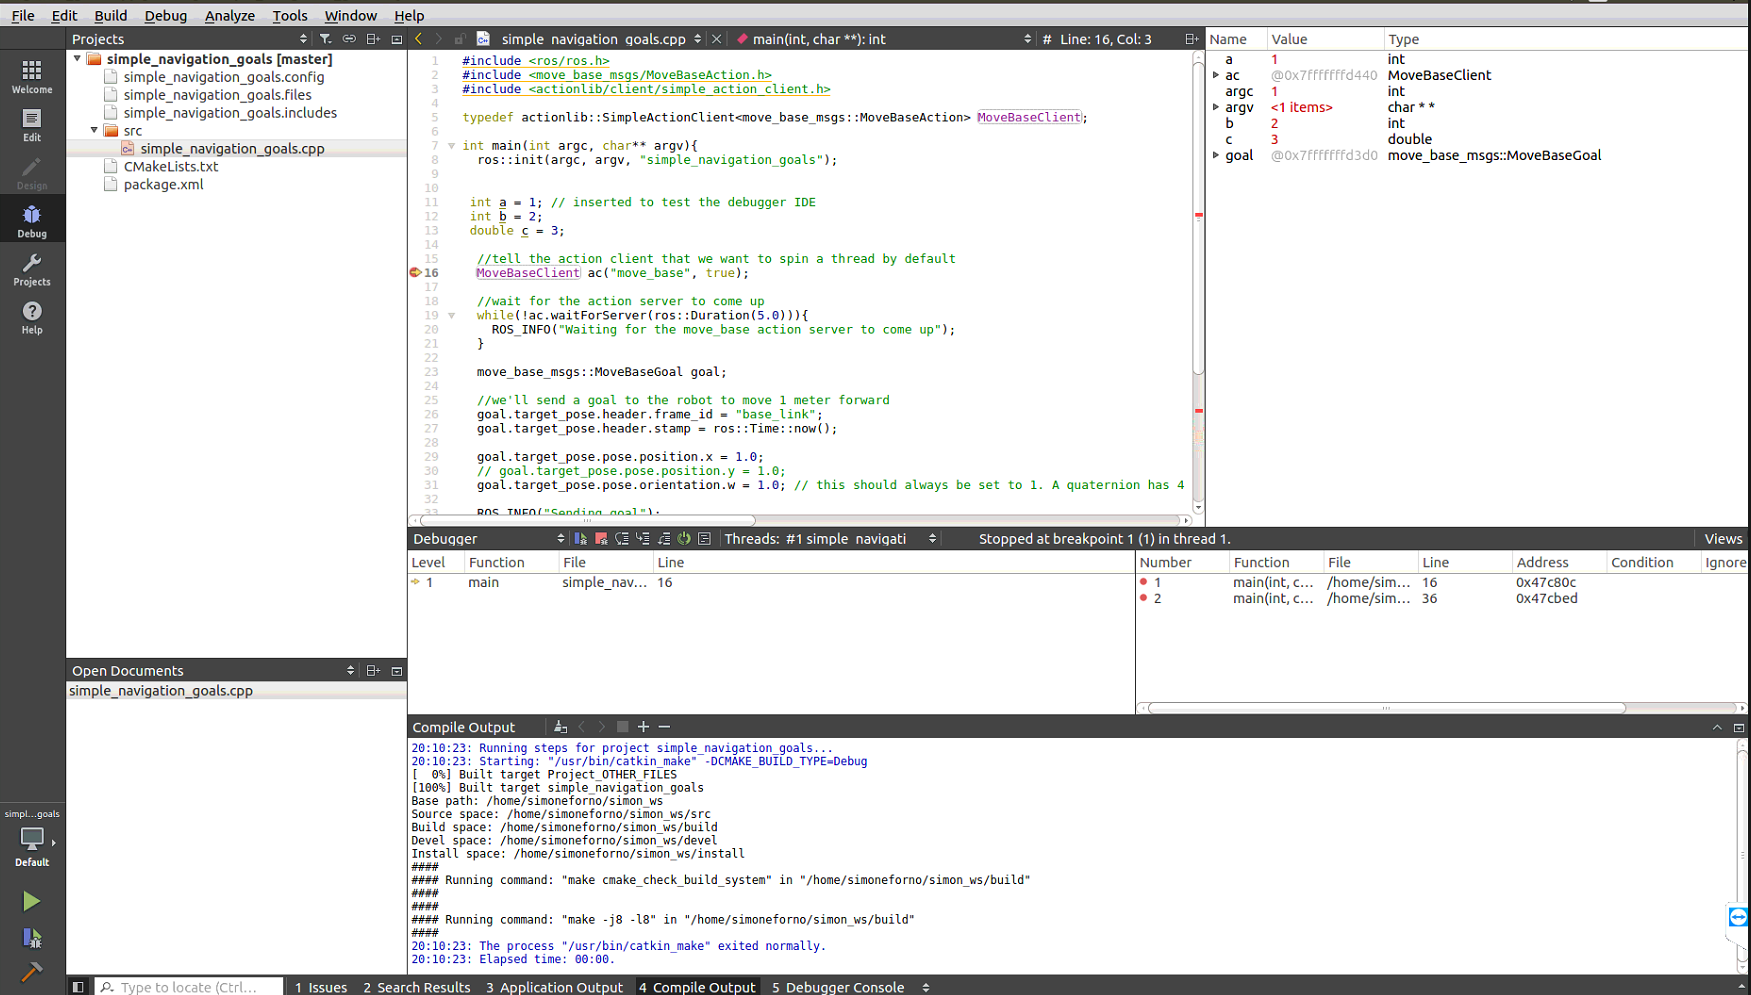
\includegraphics[width=1.1\textwidth]{figures/big_window.png}
	\caption{Debugger in action}
	\label{fig:overall}
\end{figure}


\end{document}



% == TABLE ==
%begin{table}[h!]
 % \centering
  %\caption{Caption for the table.}
 % \label{tab:table1}
 % \begin{tabular}{ccc}
 %   \toprule
  %  Some & actual & content\\
   % \midrule
   % prettifies & the & content\\
   % as & well & as\\
  %  using & the & booktabs package\\
  %   \bottomrule
  %\end{tabular}
%\end{table}


% === ALGORITHM == 

\iffalse % multi-comment tool
\begin{algorithm}[!h]
   \caption{Kirsch, Rohig algorithm}
    \begin{algorithmic}[1]
    	\State $St-1 = St$
        \For{$i = 1$ to $N$} \Comment{With N the number of particles in the filter set by maxparticle parameter}
            \State $Spread $ $particles$ $in$ $the$ $anchorbox$ $with$ $equations$ $1)$ $and$ $2)$ $of$ $[3]$ \Comment{This step is called $Global$ $Localization$}
            
            \State $xt[n] = p(xt|xt-1,ut)$ \Comment{Motion update - sample the particles from the motion update of the robot and move forward to estimate the error model functions}
            
        	\State $wt[n] = p(dnanoLOC|si)*p(dlaser|si)$ \Comment{Measurement update - si are the particles set with i the i-th index}
        	\State $St = St + <xt,wt>$ \Comment{add the state and weight to the total state space}
        	
        	\State $Perform$ $resampling$
        \EndFor
    \State $Return$ $St$

\end{algorithmic}
\end{algorithm}
\fi


\iffalse

\begin{figure}[!htb]
    \centering
    \begin{minipage}{.5\textwidth}
        \centering
        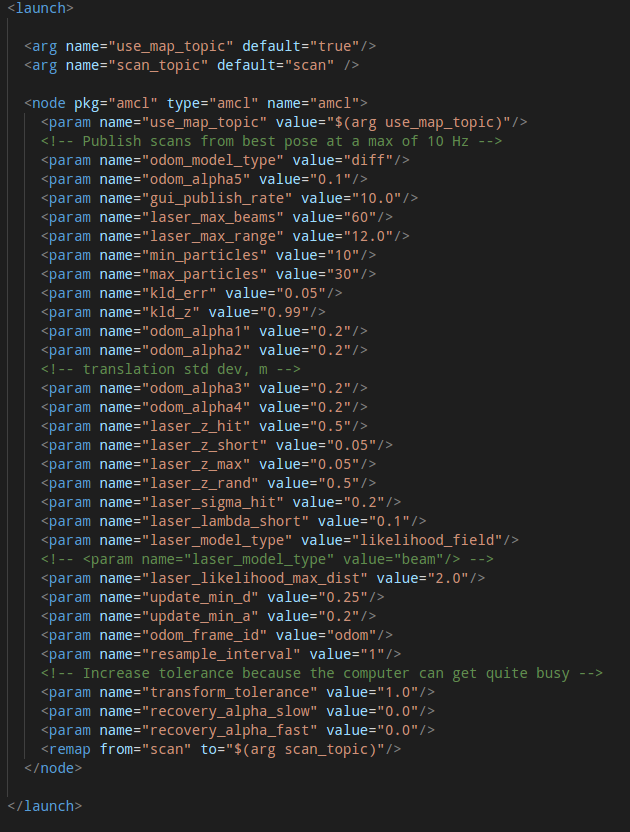
\includegraphics[width=0.7\linewidth, height=0.2\textheight]{figures/amcl_param}
        \caption{The $amcl$ tunable parameters}
        \label{fig:amcl_param}
    \end{minipage}%
    \begin{minipage}{0.5\textwidth}
        \centering
        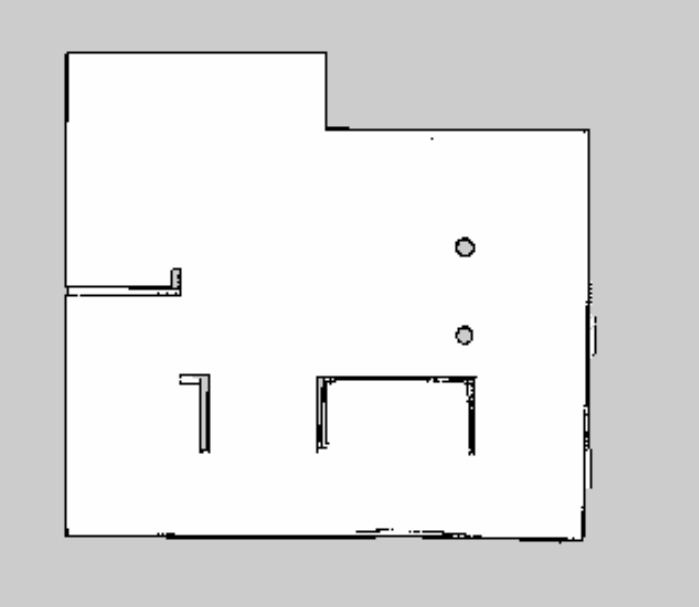
\includegraphics[width=0.7\linewidth, height=0.2\textheight]{figures/my_amcl_gmapping}
        \caption{Result of the Gmapping for the simple indoor environment}
        \label{fig:myamcl_map}
    \end{minipage}
 \end{figure}
 
 
 
 \begin{figure}[!htb]
	\center
	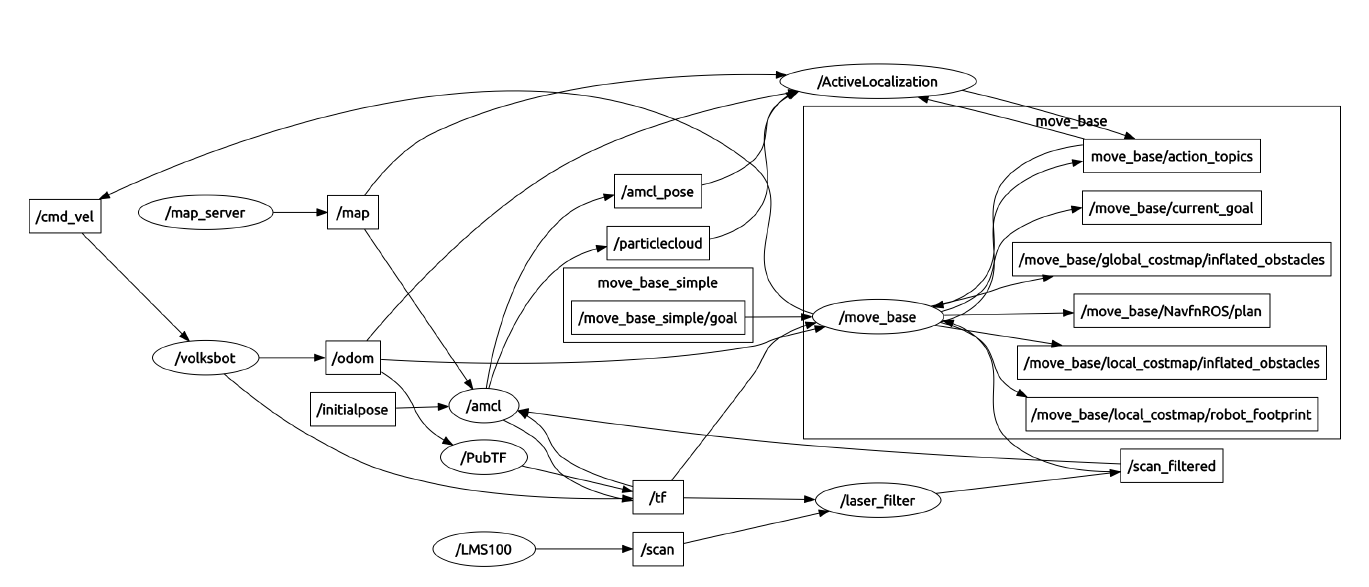
\includegraphics[width=1\textwidth]{figures/active_localization_node.png}
	\caption{An example of an active localization node}
	\label{fig:active_locnode}
\end{figure}


% underscore symbol {\_}


\fi